\chapter{Numerical results} \label{chap:results}
In this chapter we present some numerical results. The convergence of higher 
order methods applied to the Navier-Stokes equations is tested, first in space, 
then in time. Then another spatial comparison test between the upwind method 
and the TVD methods is performed using a channel flow. After that the results 
from the backward facing step test using the RANS equations are shown and 
compared to those from the CFL3D code \cite{web:nasa}. Next, a turbulent 
channel flow with two small cavities is studied and at last a coupled free-flow 
and porous-medium flow problem is analysed, varying the permeability of the 
porous-medium.\\
In all the tests the gravity has been neglected.
%
\section{Navier-Stokes tests}
\subsection{Space convergence} \label{subsec:conv}
We want to test the spatial convergence order of the $L^2$-error of the 
solution of the Navier-Stokes equations, comparing the results obtained with 
the upwind method \eqref{eq:upwind} and the TVD methods described in 
Subsection~\ref{subsec:tvd}.\\
We consider a steady version of the 
equations~\eqref{eq:nsmass}--\eqref{eq:nsmom}:
\begin{align}
	\label{eq:nssteadymass} \nabla \cdot \mathbf{v} -h = 0&\\
	\label{eq:nssteadymom} \nabla \cdot (\mathbf{v} \mathbf{v}^\mathrm{T}) - 
	\nabla \cdot (\nu \nabla \mathbf{v}) + \frac{1}{\varrho}\nabla p  
	-\mathbf{f} = \mathbf{0}&
\end{align}
We neglect the gravity, but we take into account two possible source terms 
$h$ and $\mathbf{f}$. Moreover, for the sake of simplicity, we consider here 
all the quantities appearing in the equations to be non-dimensional.
%
\subsubsection{Sin-Cos test}
Let us solve the equations~\eqref{eq:nssteadymass}--\eqref{eq:nssteadymom} over 
a two-dimensional unit domain $\Omega=(0,1)^2$, with the following source terms:
\begin{align}
	h &= 0,\\
	\mathbf{f} &= [-2\nu \cos(x) \sin(y), \; 2\nu \cos(y) \sin(x)]^\mathrm{T},
\end{align}
so that, choosing $\varrho=1$, the analytical solution, depicted in 
Figure~\ref{fig:sincosexact}, is given by
\begin{align}
\label{eq:uexsin}	u_\text{ex}(x,y) &= -\cos(x)\sin(y)\\
	v_\text{ex}(x,y) &= \sin(x)\cos(y)\\
\label{eq:pexsin}	p_\text{ex}(x,y) &= -\frac{\cos(2x)+\sin(2y)}{4}
\end{align}
Dirichlet boundary conditions for the velocity are applied on the whole 
boundary $\partial \Omega$ using the exact solution. Because of this choice, 
the pressure appears in the problem only in the momentum equation 
\eqref{eq:nssteadymom}, under the sign of gradient. Thus in the numerical 
solution it would be defined up to a constant, so we fix its value at one point 
in the domain in order to match the exact solution \eqref{eq:pexsin}.
\begin{figure}
	\centering
	\subfloat{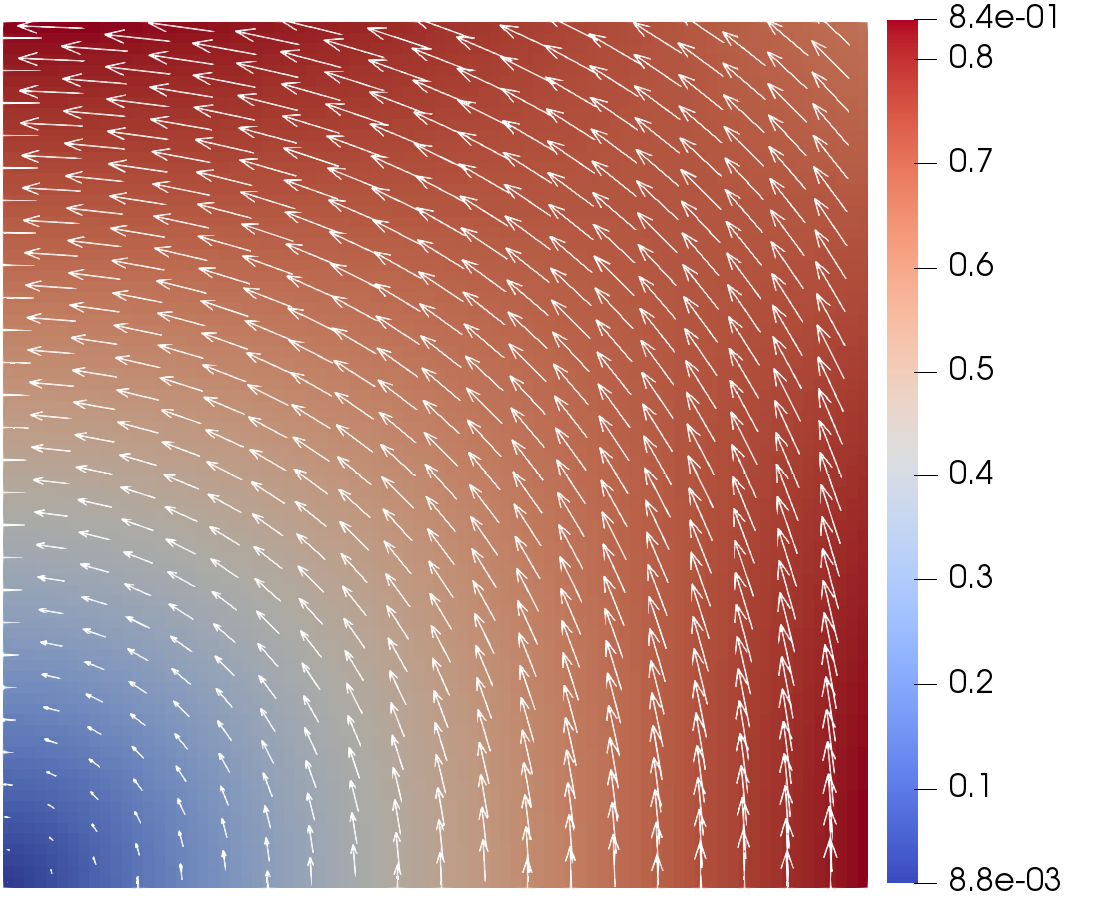
\includegraphics[width=0.5\textwidth]{sincos_exact_v_report.png}}
	\subfloat{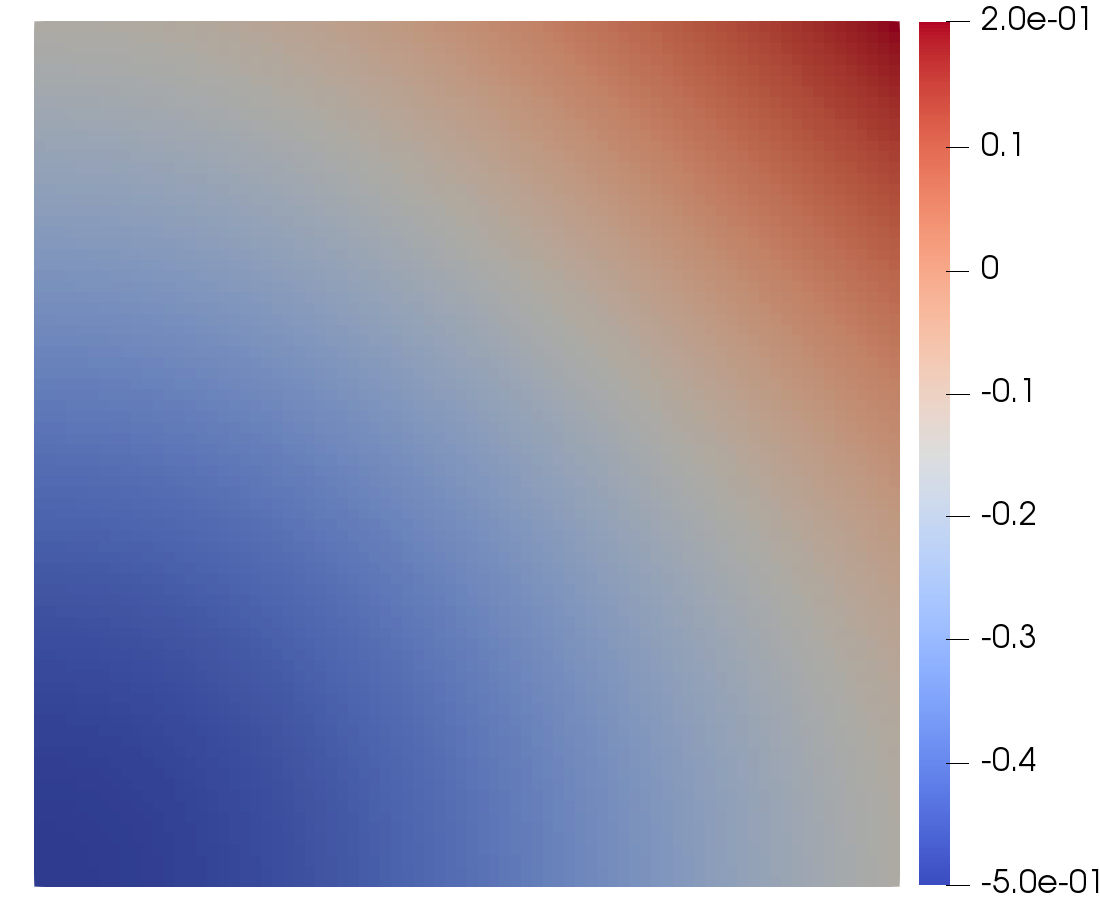
\includegraphics[width=0.5\textwidth]{sincos_exact_p_report.png}}
	\caption[Exact solution of the Sin-Cos test]{Exact solution of the Sin-Cos 
	test \eqref{eq:uexsin}--\eqref{eq:pexsin}. On the left the magnitude of the 
	velocity field, on the right the 
	pressure field.}
	\label{fig:sincosexact}
\end{figure}

The problem is solved over a sequence of five uniform grids, starting from 
$\num{4x4}$ cells and each time halving their size. Both the cases of $\nu=1$ 
and $\nu=\num{e-3}$ are considered, that correspond to $Re=1$ and $Re=\num{e3}$ 
respectively. In Figure~\ref{fig:sin_err} the errors computed are reported 
depending on the square root of the number of cells, while in 
Tables~\ref{tab:sin_lre}--\ref{tab:sin_hre} we can compare directly the 
convergence orders for the different differencing schemes.
\begin{figure}
	\centering
	\subfloat[Upwind, $Re = 1$]{
		% This file was created by matlab2tikz.
%
\definecolor{mycolor1}{rgb}{0.00000,0.44700,0.74100}%
\definecolor{mycolor2}{rgb}{0.85000,0.32500,0.09800}%
\definecolor{mycolor3}{rgb}{0.92900,0.69400,0.12500}%
%
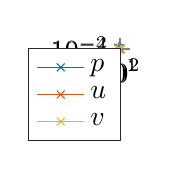
\begin{tikzpicture}

\begin{axis}[%
width=0.951\figwidth,
height=0.75\figwidth,
at={(0\figwidth,0\figwidth)},
scale only axis,
xmode=log,
xmin=4,
xmax=100,
xminorticks=true,
ymode=log,
ymin=1e-05,
ymax=0.1,
yminorticks=true,
axis background/.style={fill=white},
legend style={at={(0.97,0.97)}, anchor=north east, legend cell align=left, align=left, draw=white!15!black}
]
\addplot [color=mycolor1, mark=x, mark options={solid, mycolor1}]
  table[row sep=crcr]{%
4	0.0377253281\\
8	0.016292839\\
16	0.00647505826\\
32	0.00277859939\\
64	0.00131783073\\
};
\addlegendentry{$p$}

\addplot [color=mycolor2, mark=x, mark options={solid, mycolor2}]
  table[row sep=crcr]{%
4	0.00100309389\\
8	0.000409725552\\
16	0.000134946447\\
32	5.06672786e-05\\
64	2.29407924e-05\\
};
\addlegendentry{$u$}

\addplot [color=mycolor3, mark=x, mark options={solid, mycolor3}]
  table[row sep=crcr]{%
4	0.000631316968\\
8	0.000278812074\\
16	0.00010907144\\
32	4.76177485e-05\\
64	2.28652417e-05\\
};
\addlegendentry{$v$}

\addplot [color=white!70!black, forget plot]
  table[row sep=crcr]{%
4	0.00025\\
100	1e-05\\
};
\addplot [color=white!70!black, forget plot]
  table[row sep=crcr]
	\subfloat[Upwind, $Re = \num{e3}$]{
		% This file was created by matlab2tikz.
%
\definecolor{mycolor1}{rgb}{0.00000,0.44700,0.74100}%
\definecolor{mycolor2}{rgb}{0.85000,0.32500,0.09800}%
\definecolor{mycolor3}{rgb}{0.92900,0.69400,0.12500}%
%
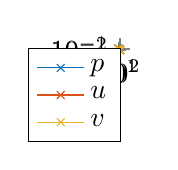
\begin{tikzpicture}

\begin{axis}[%
width=0.951\figwidth,
height=0.75\figwidth,
at={(0\figwidth,0\figwidth)},
scale only axis,
xmode=log,
xmin=4,
xmax=100,
xminorticks=true,
ymode=log,
ymin=0.00266295649,
ymax=0.1,
yminorticks=true,
axis background/.style={fill=white},
legend style={at={(0.97,0.97)}, anchor=north east, legend cell align=left, align=left}
]
\addplot [color=mycolor1, mark=x, mark options={solid, mycolor1}]
  table[row sep=crcr]{%
4	0.0596083589\\
8	0.0364982308\\
16	0.0196434526\\
32	0.00962257784\\
64	0.00434161729\\
};
\addlegendentry{$p$}

\addplot [color=mycolor2, mark=x, mark options={solid, mycolor2}]
  table[row sep=crcr]{%
4	0.0339372138\\
8	0.0206751686\\
16	0.011131246\\
32	0.00559430586\\
64	0.00266295649\\
};
\addlegendentry{$u$}

\addplot [color=mycolor3, mark=x, mark options={solid, mycolor3}]
  table[row sep=crcr]{%
4	0.0347600515\\
8	0.0213374017\\
16	0.0114856296\\
32	0.00577467407\\
64	0.00275450966\\
};
\addlegendentry{$v$}

\addplot [color=white!70!black, forget plot]
  table[row sep=crcr]{%
4	0.06657391225\\
100	0.00266295649\\
};
\addplot [color=white!70!black, forget plot]
  table[row sep=crcr]\\
	\subfloat[Min-Mod, $Re = 1$]{
		% This file was created by matlab2tikz.
%
\definecolor{mycolor1}{rgb}{0.00000,0.44700,0.74100}%
\definecolor{mycolor2}{rgb}{0.85000,0.32500,0.09800}%
\definecolor{mycolor3}{rgb}{0.92900,0.69400,0.12500}%
%
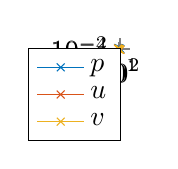
\begin{tikzpicture}

\begin{axis}[%
width=0.951\figwidth,
height=0.75\figwidth,
at={(0\figwidth,0\figwidth)},
scale only axis,
xmode=log,
xmin=4,
xmax=100,
xminorticks=true,
ymode=log,
ymin=1e-05,
ymax=0.1,
yminorticks=true,
axis background/.style={fill=white},
legend style={at={(0.97,0.97)}, anchor=north east, legend cell align=left, align=left}
]
\addplot [color=mycolor1, mark=x, mark options={solid, mycolor1}]
  table[row sep=crcr]{%
4	0.0201961443\\
8	0.00658170291\\
16	0.00181646151\\
32	0.000558641084\\
64	0.000188245776\\
};
\addlegendentry{$p$}

\addplot [color=mycolor2, mark=x, mark options={solid, mycolor2}]
  table[row sep=crcr]{%
4	0.00148598782\\
8	0.00053497283\\
16	0.000150385476\\
32	3.95894587e-05\\
64	1.01636468e-05\\
};
\addlegendentry{$u$}

\addplot [color=mycolor3, mark=x, mark options={solid, mycolor3}]
  table[row sep=crcr]{%
4	0.00119526142\\
8	0.00045470553\\
16	0.000138075359\\
32	3.80865907e-05\\
64	1.00057526e-05\\
};
\addlegendentry{$v$}

\addplot [color=white!70!black, forget plot]
  table[row sep=crcr]{%
4	0.00025\\
100	1e-05\\
};
\addplot [color=white!70!black, forget plot]
  table[row sep=crcr]
	\subfloat[Min-Mod, $Re = \num{e3}$]{
		% This file was created by matlab2tikz.
%
\definecolor{mycolor1}{rgb}{0.00000,0.44700,0.74100}%
\definecolor{mycolor2}{rgb}{0.85000,0.32500,0.09800}%
\definecolor{mycolor3}{rgb}{0.92900,0.69400,0.12500}%
%
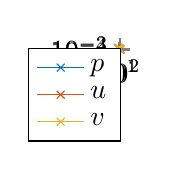
\begin{tikzpicture}

\begin{axis}[%
width=0.951\figwidth,
height=0.75\figwidth,
at={(0\figwidth,0\figwidth)},
scale only axis,
xmode=log,
xmin=4,
xmax=100,
xminorticks=true,
ymode=log,
ymin=0.0001,
ymax=0.0206930353,
yminorticks=true,
axis background/.style={fill=white},
legend style={at={(0.97,0.97)}, anchor=north east, legend cell align=left, align=left}
]
\addplot [color=mycolor1, mark=x, mark options={solid, mycolor1}]
  table[row sep=crcr]{%
4	0.0206930353\\
8	0.0102262223\\
16	0.00364544433\\
32	0.000812298263\\
64	0.000257143964\\
};
\addlegendentry{$p$}

\addplot [color=mycolor2, mark=x, mark options={solid, mycolor2}]
  table[row sep=crcr]{%
4	0.0130268788\\
8	0.00605072242\\
16	0.00243635311\\
32	0.000918041806\\
64	0.000338134479\\
};
\addlegendentry{$u$}

\addplot [color=mycolor3, mark=x, mark options={solid, mycolor3}]
  table[row sep=crcr]{%
4	0.0129926934\\
8	0.00750558766\\
16	0.0037160882\\
32	0.00148526754\\
64	0.000512917943\\
};
\addlegendentry{$v$}

\addplot [color=white!70!black, forget plot]
  table[row sep=crcr]{%
4	0.0025\\
100	0.0001\\
};
\addplot [color=white!70!black, forget plot]
  table[row sep=crcr]\\
	\subfloat[Van Leer, $Re = 1$]{
		% This file was created by matlab2tikz.
%
\definecolor{mycolor1}{rgb}{0.00000,0.44700,0.74100}%
\definecolor{mycolor2}{rgb}{0.85000,0.32500,0.09800}%
\definecolor{mycolor3}{rgb}{0.92900,0.69400,0.12500}%
%
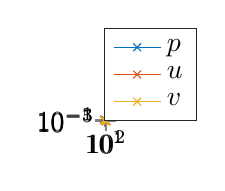
\begin{tikzpicture}

\begin{axis}[%
width=0.951\figwidth,
height=0.75\figwidth,
at={(0\figwidth,0\figwidth)},
scale only axis,
xmode=log,
xmin=4,
xmax=100,
xminorticks=true,
ymode=log,
ymin=8.63199669e-06,
ymax=0.1,
yminorticks=true,
axis background/.style={fill=white},
legend style={at={(0.03,0.03)}, anchor=south west, legend cell align=left, align=left, draw=white!15!black}
]
\addplot [color=mycolor1, mark=x, mark options={solid, mycolor1}]
  table[row sep=crcr]{%
4	0.017335487\\
8	0.0062618753\\
16	0.00193371119\\
32	0.000605597659\\
64	0.000196206927\\
};
\addlegendentry{$p$}

\addplot [color=mycolor2, mark=x, mark options={solid, mycolor2}]
  table[row sep=crcr]{%
4	0.00136409678\\
8	0.000476275877\\
16	0.000131606902\\
32	3.41242821e-05\\
64	8.66824542e-06\\
};
\addlegendentry{$u$}

\addplot [color=mycolor3, mark=x, mark options={solid, mycolor3}]
  table[row sep=crcr]{%
4	0.00114596769\\
8	0.000417513208\\
16	0.000122988533\\
32	3.32359157e-05\\
64	8.63199669e-06\\
};
\addlegendentry{$v$}

\addplot [color=white!70!black, forget plot]
  table[row sep=crcr]{%
4	0.00021579991725\\
100	8.63199669e-06\\
};
\addplot [color=white!70!black, forget plot]
  table[row sep=crcr]
	\subfloat[Van Leer, $Re = \num{e3}$]{
		% This file was created by matlab2tikz.
%
\definecolor{mycolor1}{rgb}{0.00000,0.44700,0.74100}%
\definecolor{mycolor2}{rgb}{0.85000,0.32500,0.09800}%
\definecolor{mycolor3}{rgb}{0.92900,0.69400,0.12500}%
%
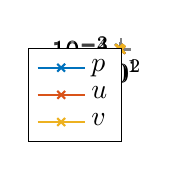
\begin{tikzpicture}

\begin{axis}[%
width=0.951\figwidth,
height=0.75\figwidth,
at={(0\figwidth,0\figwidth)},
scale only axis,
xmode=log,
xmin=4,
xmax=100,
xminorticks=true,
ymode=log,
ymin=0.0001,
ymax=0.01454297,
yminorticks=true,
axis background/.style={fill=white},
legend style={at={(0.97,0.97)}, anchor=north east, legend cell align=left, align=left}
]
\addplot [color=white!70!black, forget plot, line width=0.75pt]
  table[row sep=crcr]{%
4	0.0025\\
100	0.0001\\
};
\addplot [color=white!70!black, forget plot, line width=0.75pt]
  table[row sep=crcr]{%
4	0.0625\\
100	0.0001\\
};
\addplot [color=mycolor1, mark=x, mark options={solid, mycolor1}, line width=0.75pt]
  table[row sep=crcr]{%
4	0.01454297\\
8	0.00653869074\\
16	0.00224775854\\
32	0.0005196908\\
64	0.000249600967\\
};
\addlegendentry{$p$}

\addplot [color=mycolor2, mark=x, mark options={solid, mycolor2}, line width=0.75pt]
  table[row sep=crcr]{%
4	0.0107200353\\
8	0.00466675248\\
16	0.00177426299\\
32	0.000645881865\\
64	0.000238530337\\
};
\addlegendentry{$u$}

\addplot [color=mycolor3, mark=x, mark options={solid, mycolor3}, line width=0.75pt]
  table[row sep=crcr]
	\caption[$L^2$-errors for the Sin-Cos test]{$L^2$-errors for the Sin-Cos 
	test depending on the square root of the number of cells in the grid. 
	The grey lines are the reference lines for the first-order and second-order 
	convergence.}
	\label{fig:sin_err}
\end{figure}

\begin{table}
	\centering
	\[
	\begin{array}{c|ccc}
	\toprule
	& \text{Upwind} & \text{Min-Mod} & \text{Van Leer} \\ 
	\midrule
	p & 1.008 & 1.569 & 1.626\\
	v_x & 1.143 & 1.962 & 1.977\\
	v_y & 1.058 & 1.928 & 1.945\\
	\bottomrule
	\end{array}
	\]
	\caption[Convergence orders with $Re = 1$ for the Sin-Cos 
	test]{Convergence orders with $Re = 1$ for the Sin-Cos test. They are 
	computed considering the last two refinements of the grid.}
	\label{tab:sin_lre}
	\[
	\begin{array}{c|ccc}
	\toprule
	& \text{Upwind} & \text{Min-Mod} & \text{Van Leer} \\ 
	\midrule
	p & 1.148 & 1.659 & 1.058\\
	v_x & 1.071 & 1.441 & 1.437\\
	v_y & 1.068 & 1.533 & 1.560\\
	\bottomrule
	\end{array}
	\]
	\caption[Convergence orders with $Re = \num{e3}$ for the Sin-Cos 
	test]{Convergence orders with $Re = \num{e3}$ for the Sin-Cos test. 
	They are computed considering the last two refinements of the grid.}
	\label{tab:sin_hre}
\end{table}

We observe, as expected, a better behaviour of the TVD methods with respect to 
the upwind method. In Table~\ref{tab:sin_lre} we can see that at $Re=1$ the 
formers show a full second order convergence for the velocity, while for the 
rate is a bit lower; the latter instead shows a first for all the variables. At 
$Re=\num{e3}$ a slight decrease of the rates of the TVD methods occurs also for 
the velocities, but they remain higher then the ones of the upwind method. In 
Table~\ref{tab:sin_hre} we observe a convergence order of 1 for the pressure 
using the Van Leer flux limiter, but looking at Figure~\ref{fig:sin_err} we can 
see that the global trend indicates a convergence of higher order. Moreover it 
can be observed how, thanks to the faster convergence, on the same grid the 
absolute values of the errors reach smaller values using the TVD methods. 
Between the Min-Mod and Van Leer flux limiter it is hard to say which performs 
better, the results are very similar.

Analogous tests with other analytical solutions are reported in the 
Appendix~\ref{app:conv}. They show always a better convergence of the TVD 
methods with respect to the upwind method, but in some cases the convergence 
order of pressure and velocity behave differently.
%
\subsection{Time convergence}
We test the time convergence of the $L^\infty(0,T;L^2(\Omega))$ norm of the 
error of the solution of the Navier-Stokes equations, comparing the results 
obtained with the BE method \eqref{eq:be} and the BDF2 method \eqref{eq:bdf2}.\\
We consider the unsteady version of the 
equations~\eqref{eq:nssteadymass}--\eqref{eq:nssteadymom}:
\begin{align}
	\label{eq:nsunsteadymass} \nabla \cdot \mathbf{v} -h = 0&\\
	\label{eq:nsunsteadymom} \frac{\partial \mathbf{v}}{\partial t} +\nabla 
	\cdot (\mathbf{v} \mathbf{v}^\mathrm{T}) - 
	\nabla \cdot (\nu \nabla \mathbf{v}) + \frac{1}{\varrho}\nabla p  
	-\mathbf{f} = \mathbf{0}&
\end{align}
Again the gravity is neglected and two possible sources $h$ and $\mathbf{f}$ 
are taken into account, moreover all the quantities are considered to be 
non-dimensional.
%
\subsubsection{Unsteady Sin-Cos test}
Let us solve the equations~\eqref{eq:nsunsteadymass}--\eqref{eq:nsunsteadymom} 
over a two dimensional unit domain $\Omega=(0,1)^2$ and in the time interval 
$(0,T)$, with $T=1$. We use the following source terms:
\begin{align}
h &= 0,\\
\mathbf{f} &= 2\Big(\frac{\cos(2t)}{\varrho} + \nu \sin(2t)\Big)[- \cos(x) 
\sin(y), \; 
\cos(y) \sin(x)]^\mathrm{T},
\end{align}
so that, choosing $\varrho=1$, the analytical solution is given by
\begin{align}
\label{eq:uexunssin}	u_\text{ex}(x,y) &= -\cos(x)\sin(y)\sin(2t)\\
v_\text{ex}(x,y) &= \sin(x)\cos(y)\sin(2t)\\
\label{eq:pexunssin}	p_\text{ex}(x,y) &= 
-\frac{\cos(2x)+\sin(2y)}{4}\sin^2(2t),
\end{align}
so it is equal to \eqref{eq:uexsin}--\eqref{eq:pexsin}, used in the steady test 
for the space convergence, except for the modulation over time. We choose 
$\nu=0.1$, so that $Re=10$. Dirichlet boundary conditions for the velocity are 
applied on the whole boundary $\partial \Omega$ using the exact solution. 
Pressure is again fixed  at one point in order to match the exact solution 
\eqref{eq:pexunssin}.

The problem is solved seven times subdividing the time interval $(0,T)$ into 
uniform time-steps and each time time doubling their number, starting from a 
single time-step. Uniform grids of $\num{40x40}$ and $\num{80x80}$ cells are 
employed and as a differencing scheme the TVD method with the Van Leer flux 
limiter \eqref{eq:vl} is used. From Figure~\ref{fig:timeerr} we observe that, 
as expected, the BE method shows a first-order convergence, while the BDF2 
method is of second order. Moreover we notice that, with a grid of 
$\num{40x40}$ cells, in the last refinement the error with the BDF2 method does 
not decrease anymore. This happens because the spatial error becomes 
dominant, indeed refining the grid the convergence order is restored entirely 
for the pressure and almost for the velocity.
\begin{figure}
	\centering
	\subfloat{% This file was created by matlab2tikz.
%
\definecolor{mycolor1}{rgb}{0.00000,0.44700,0.74100}%
\definecolor{mycolor2}{rgb}{0.85000,0.32500,0.09800}%
\definecolor{mycolor3}{rgb}{0.92900,0.69400,0.12500}%
%
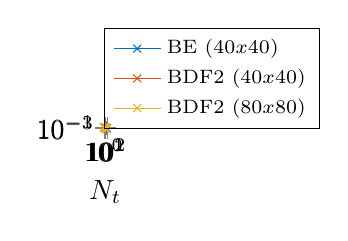
\begin{tikzpicture}

\begin{axis}[%
width=0.99\figwidth,
height=0.8\figwidth,
at={(0\figwidth,0\figwidth)},
scale only axis,
xmode=log,
xmin=1,
xmax=100,
xminorticks=true,
xlabel={$N_t$},
ymode=log,
ymin=0.0001,
ymax=1,
yminorticks=true,
%ylabel style={font=\scriptsize},
%ylabel={$L^\infty$-error},
axis background/.style={fill=white},
legend style={at={(0.03,0.03)}, anchor=south west, legend cell align=left, fill=none,
align=left, font=\scriptsize}
]
\addplot [color=mycolor1, mark=x, mark options={solid, mycolor1}]
  table[row sep=crcr]{%
1	2.91e-1\\
2	1.619e-1\\
4	8.07e-2\\
8	4.17e-2\\
16	2.1e-2\\
32	1.054e-2\\
64	5.31e-3\\
};
\addlegendentry{BE ($\num{40x40}$)}

\addplot [color=mycolor2, mark=x, mark options={solid, mycolor2}]
  table[row sep=crcr]{%
1	2.91e-1\\
2	1e-1\\
4	2.686e-2\\
8	6.81e-3\\
16	1.7e-3\\
32	4.23e-4\\
64	3.816e-4\\
};
\addlegendentry{BDF2 ($\num{40x40}$)}

\addplot [color=mycolor3, mark=x, mark options={solid, mycolor3}]
  table[row sep=crcr]{%
1	2.91e-1\\
2	1e-1\\
4	2.686e-2\\
8	6.814e-3\\
16	1.704e-3\\
32	4.258e-4\\
64	1.347e-4\\
};
\addlegendentry{BDF2 ($\num{80x80}$)}

\addplot [color=white!70!black, forget plot]
  table[row sep=crcr]{%
1	1\\
100	0.01\\
};
\addplot [color=white!70!black, forget plot]
  table[row sep=crcr]
	\subfloat{% This file was created by matlab2tikz.
%
\definecolor{mycolor1}{rgb}{0.00000,0.44700,0.74100}%
\definecolor{mycolor2}{rgb}{0.85000,0.32500,0.09800}%
\definecolor{mycolor3}{rgb}{0.92900,0.69400,0.12500}%
%
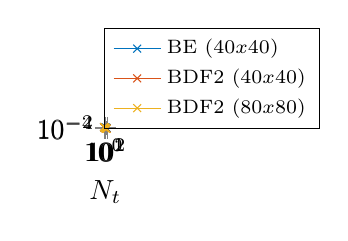
\begin{tikzpicture}

\begin{axis}[%
width=0.99\figwidth,
height=0.8\figwidth,
at={(0\figwidth,0\figwidth)},
scale only axis,
xmode=log,
xmin=1,
xmax=100,
xminorticks=true,
xlabel={$N_t$},
ymode=log,
ymin=1e-5,
ymax=1e-1,
yminorticks=true,
%ylabel style={font=\scriptsize},
%ylabel={$L^\infty$-error},
axis background/.style={fill=white},
legend style={at={(0.03,0.03)}, anchor=south west, legend cell align=left, fill=none,
align=left, font=\scriptsize}
]
\addplot [color=mycolor1, mark=x, mark options={solid, mycolor1}]
  table[row sep=crcr]{%
1	5.516e-2\\
2	3.043e-2\\
4	1.607e-2\\
8	8.216e-3\\
16	4.12e-3\\
32	2.03e-3\\
64	9.712e-4\\
};
\addlegendentry{BE ($\num{40x40}$)}

\addplot [color=mycolor2, mark=x, mark options={solid, mycolor2}]
  table[row sep=crcr]{%
1	5.516e-2\\
2	1.645e-2\\
4	4.8e-3\\
8	1.21e-3\\
16	2.85e-4\\
32	1.3e-4\\
64	1.278e-4\\
};
\addlegendentry{BDF2 ($\num{40x40}$)}

\addplot [color=mycolor3, mark=x, mark options={solid, mycolor3}]
  table[row sep=crcr]{%
1	5.42e-2\\
2	1.647e-2\\
4	4.83e-3\\
8	1.231e-3\\
16	3.024e-4\\
32	7.061e-5\\
64	3.6e-5\\
};
\addlegendentry{BDF2 ($\num{80x80}$)}

\addplot [color=white!70!black, forget plot]
  table[row sep=crcr]{%
1	0.1\\
100	0.001\\
};
\addplot [color=white!70!black, forget plot]
  table[row sep=crcr]
	\caption[$L^\infty(0,T;L^2(\Omega))$-errors for the unsteady Sin-Cos 
	test]{$L^\infty(0,T;L^2(\Omega))$-errors for the unsteady Sin-Cos test 
	depending on the number of time-steps. On the left the errors for the 
	pressure, on the right the error for the magnitude of the velocity. The 
	grey lines are the reference lines for the first-order and second-order 
	convergence.}
	\label{fig:timeerr}
\end{figure}
%
\subsection{Rough channel test}
We test the behaviour of the TVD methods compared to the upwind method solving 
the unsteady Navier-Stokes equations \eqref{eq:nsmass}--\eqref{eq:nsmom} in 
a two-dimensional channel with a rough (i.e. non-flat) lower boundary. The 
roughness consists of small evenly spaced cavities. Two different 
configurations are studied, one with shallow cavities, depicted in 
Figure~\ref{fig:roughdom}, and another with deeper cavities, depicted in 
Figure~\ref{fig:roughdomdeep}.

On the left boundary $\Gamma_\text{in}$ we set inflow boundary conditions 
\eqref{eq:inflow}, specifying an horizontal velocity
\begin{equation}
	\mathbf{v} = \mathbf{v}_\text{in} = [u_\text{in}, 0]^\mathrm{T}, \quad 
	u_\text{in} = \SI{1}{m/s}.
\end{equation}
On the lower and upper boundaries $\Gamma_w$ we set no-slip boundary conditions 
\eqref{eq:noslip}, while on the right boundary $\Gamma_\text{out}$ we set 
outflow boundary conditions \eqref{eq:outflow}, fixing the value of the pressure
\begin{equation}
	p = p_\text{ext} = \SI{1.1e5}{\pascal}.
\end{equation}
As initial conditions the velocity is set to zero everywhere, while the 
pressure is set to $p_\text{ext}$ everywhere. The density is 
$\varrho=\SI{1}{kg/m^3}$. The gravity contribution in \eqref{eq:nsmom} is 
neglected.
%
\subsubsection{Shallow cavities}
In the case of shallow cavities we use the domain in Figure~\ref{fig:roughdom} 
and we employ a uniform grid of $\num{95x50}$ cells. The problem is then solved 
over the time interval [$0,T$], with $T=\SI{10}{s}$; the initial time-step is 
$\Delta t=\SI{5e-3}{s}$, then it is adapted as explained in 
Section~\ref{sec:algeq}, allowing a maximum time-step of $\SI{0.1}{s}$. 
At first we set $\nu=\SI{5e-4}{m^2/s}$, so that $Re=\num{2e3}$. Since we do not 
have an analytical solution for this problem, we compute a \emph{reference 
solution} using the upwind method over a grid six times finer.

In Figure~\ref{fig:linecompshallow} we compare the profiles of the magnitude 
of the velocity along a section near the end of the channel, at 
$x=\SI{8.75}{m}$, i.e. at the middle of the last cavity.  The TVD solutions 
match the reference one, while the upwind solution shows a small shift, 
especially in the lower part of the channel, above the cavity. So, on a coarse 
grid, we obtain a solution that is the one we would obtain with the upwind 
method on a finer grid. In Table~\ref{tab:errshallow} we can see the $L^2$-norm 
of the errors between the coarse solutions and the reference one, computed 
along the section. As expected, the one related to the upwind method is at 
least one order of magnitude larger than the others. 
\begin{figure}
	\centering
	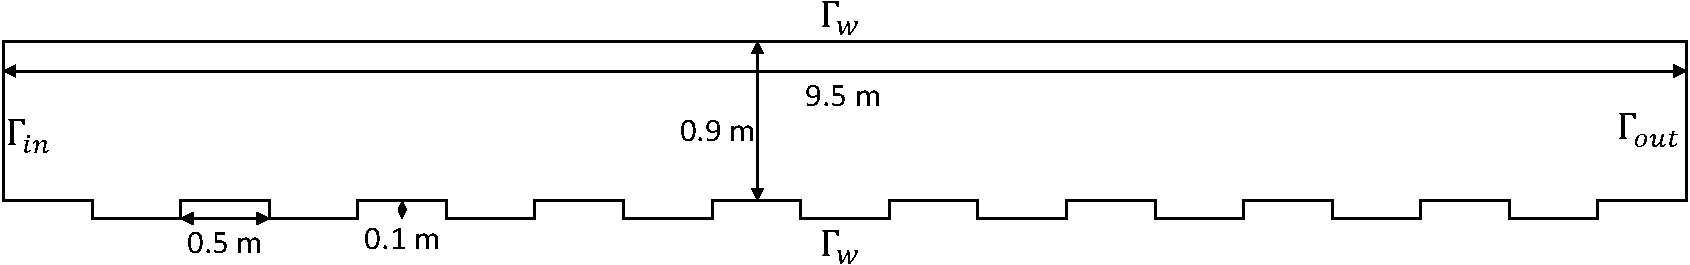
\includegraphics[width=\textwidth]{rough_domain2.pdf}
	\caption[Domain of the rough channel test with shallow cavities]{Domain of 
	the rough channel test with shallow cavities.}
	\label{fig:roughdom}
\end{figure}
\begin{figure}
	\centering
	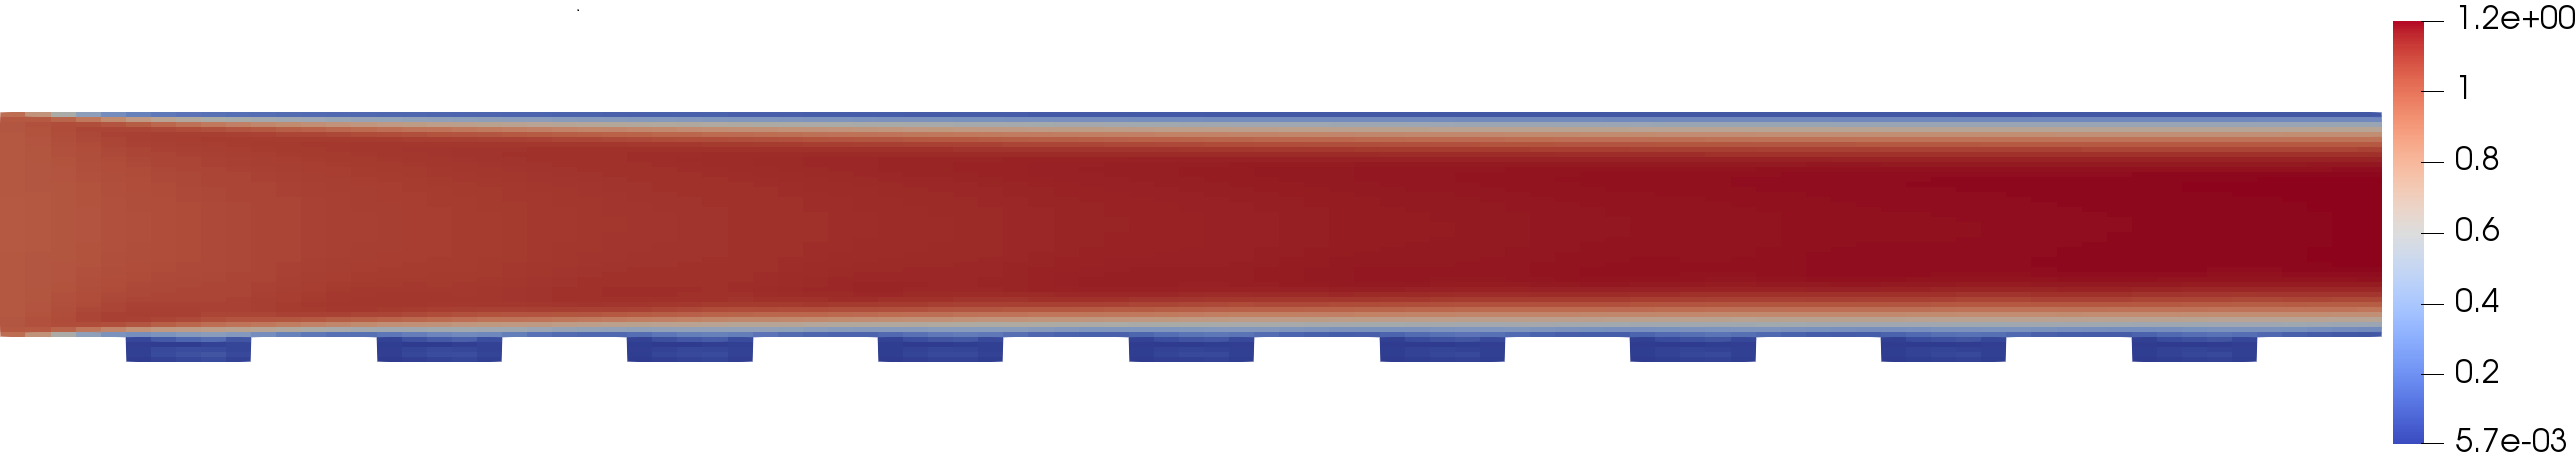
\includegraphics[width=\textwidth]{rough_channel_vl_report.png}
	\caption[Magnitude of the velocity magnitude in the rough channel test with 
	shallow cavities]{Magnitude of the velocity magnitude $[\si{m/s}]$ in the 
	rough channel test with shallow cavities at $t=\SI{10}{s}$. $Re=\num{2e3}$, 
	Van Leer flux limiter.}
	\label{fig:roughchannelvl}
\end{figure}
\begin{figure}
	\centering
	% This file was created by matlab2tikz.
%
\definecolor{mycolor1}{rgb}{0.00000,0.44700,0.74100}%
\definecolor{mycolor2}{rgb}{0.85000,0.32500,0.09800}%
\definecolor{mycolor3}{rgb}{0.92900,0.69400,0.12500}%
\definecolor{mycolor4}{rgb}{0.49400,0.18400,0.55600}%
%
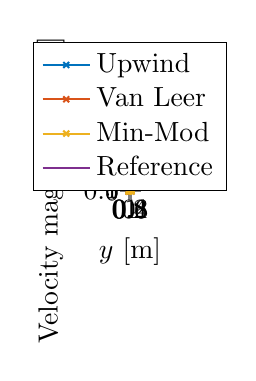
\begin{tikzpicture}

\begin{axis}[%
width=0.951\roughwidth,
height=0.75\roughheight,
at={(0\roughwidth,0\roughheight)},
scale only axis,
xmin=0,
xmax=1,
xlabel={$y$ [m]},
ymin=0,
ymax=1.25,
ylabel={Velocity magnitude [m/s]},
axis background/.style={fill=white},
legend style={at={(0.5,0.03)}, anchor=south, legend cell align=left, align=left}
]
\addplot [color=mycolor1, mark size=1.5pt, mark=x, mark options={solid, mycolor1}, line width=0.75pt]
  table[row sep=crcr]{%
0	0\\
0.01	0.0293662\\
0.03	0.050586\\
0.05	0.0374104\\
0.07	0.00830816\\
0.09	0.0878588\\
0.11	0.203537\\
0.13	0.350154\\
0.15	0.504986\\
0.17	0.648407\\
0.19	0.773425\\
0.21	0.879108\\
0.23	0.965875\\
0.25	1.0347\\
0.27	1.08726\\
0.29	1.12581\\
0.31	1.15286\\
0.33	1.17097\\
0.35	1.18249\\
0.37	1.18938\\
0.39	1.19321\\
0.41	1.19513\\
0.43	1.19595\\
0.45	1.19618\\
0.47	1.19615\\
0.49	1.19606\\
0.51	1.19602\\
0.53	1.19608\\
0.55	1.19627\\
0.57	1.19661\\
0.59	1.19708\\
0.61	1.1977\\
0.63	1.19842\\
0.65	1.19918\\
0.67	1.19986\\
0.69	1.20024\\
0.71	1.19994\\
0.73	1.19831\\
0.75	1.19437\\
0.77	1.18669\\
0.79	1.17327\\
0.81	1.15154\\
0.83	1.11834\\
0.85	1.07018\\
0.87	1.00343\\
0.89	0.914856\\
0.91	0.802051\\
0.93	0.663892\\
0.95	0.500819\\
0.97	0.314904\\
0.99	0.109749\\
1	0\\
};
\addlegendentry{Upwind}

\addplot [color=mycolor2, mark size=1.5pt, mark=x, mark options={solid, mycolor2}, line width=0.75pt]
  table[row sep=crcr]{%
0	0\\
0.01	0.0271697\\
0.03	0.0500789\\
0.05	0.0401093\\
0.07	0.00567534\\
0.09	0.0811925\\
0.11	0.199174\\
0.13	0.35443\\
0.15	0.52202\\
0.17	0.675188\\
0.19	0.804904\\
0.21	0.91139\\
0.23	0.996051\\
0.25	1.06075\\
0.27	1.10807\\
0.29	1.14103\\
0.31	1.16275\\
0.33	1.17616\\
0.35	1.18381\\
0.37	1.1877\\
0.39	1.18933\\
0.41	1.18969\\
0.43	1.18942\\
0.45	1.18894\\
0.47	1.18845\\
0.49	1.18804\\
0.51	1.18779\\
0.53	1.1877\\
0.55	1.18779\\
0.57	1.18804\\
0.59	1.18848\\
0.61	1.18909\\
0.63	1.18985\\
0.65	1.19073\\
0.67	1.19161\\
0.69	1.19229\\
0.71	1.1924\\
0.73	1.19132\\
0.75	1.18802\\
0.77	1.181\\
0.79	1.16815\\
0.81	1.14675\\
0.83	1.11359\\
0.85	1.06512\\
0.87	0.997859\\
0.89	0.908818\\
0.91	0.795828\\
0.93	0.657971\\
0.95	0.495791\\
0.97	0.311428\\
0.99	0.10845\\
1	0\\
};
\addlegendentry{Van Leer}

\addplot [color=mycolor3, mark size=1.5pt, mark=x, mark options={solid, mycolor3}, line width=0.75pt]
  table[row sep=crcr]{%
0	0\\
0.01	0.0272093\\
0.03	0.0494723\\
0.05	0.0389859\\
0.07	0.00595636\\
0.09	0.0812851\\
0.11	0.198804\\
0.13	0.353914\\
0.15	0.5204\\
0.17	0.672249\\
0.19	0.801321\\
0.21	0.907555\\
0.23	0.992249\\
0.25	1.05727\\
0.27	1.10509\\
0.29	1.13867\\
0.31	1.16106\\
0.33	1.17513\\
0.35	1.18335\\
0.37	1.18771\\
0.39	1.18968\\
0.41	1.19029\\
0.43	1.19022\\
0.45	1.18987\\
0.47	1.18946\\
0.49	1.18912\\
0.51	1.18891\\
0.53	1.18887\\
0.55	1.18899\\
0.57	1.18928\\
0.59	1.18974\\
0.61	1.19035\\
0.63	1.19112\\
0.65	1.19197\\
0.67	1.19282\\
0.69	1.19344\\
0.71	1.19347\\
0.73	1.19226\\
0.75	1.18881\\
0.77	1.18163\\
0.79	1.16863\\
0.81	1.14714\\
0.83	1.11395\\
0.85	1.06554\\
0.87	0.998402\\
0.89	0.90948\\
0.91	0.796585\\
0.93	0.658719\\
0.95	0.496437\\
0.97	0.311872\\
0.99	0.108614\\
1	0\\
};
\addlegendentry{Min-Mod}

\addplot [color=mycolor4, line width=0.75pt]
  table[row sep=crcr]{%
0	0\\
0.00166667	0.00492427\\
0.005	0.0138838\\
0.00833333	0.0219483\\
0.0116667	0.0291114\\
0.015	0.0353663\\
0.0183333	0.0407062\\
0.0216667	0.0451241\\
0.025	0.0486134\\
0.0283333	0.051167\\
0.0316667	0.0527786\\
0.035	0.0534416\\
0.0383333	0.0531503\\
0.0416667	0.0518985\\
0.045	0.0496806\\
0.0483333	0.0464911\\
0.0516667	0.042324\\
0.055	0.037174\\
0.0583333	0.0310358\\
0.0616667	0.0239061\\
0.065	0.0157914\\
0.0683333	0.00678684\\
0.0716667	0.00421506\\
0.075	0.0150977\\
0.0783333	0.0273447\\
0.0816667	0.0407005\\
0.085	0.0551595\\
0.0883333	0.0707355\\
0.0916667	0.0874415\\
0.095	0.105279\\
0.0983333	0.124233\\
0.101667	0.144291\\
0.105	0.165438\\
0.108333	0.187646\\
0.111667	0.210875\\
0.115	0.23507\\
0.118333	0.260158\\
0.121667	0.286047\\
0.125	0.312628\\
0.128333	0.33978\\
0.131667	0.367367\\
0.135	0.395245\\
0.138333	0.42327\\
0.141667	0.451298\\
0.145	0.479192\\
0.148333	0.506829\\
0.151667	0.534103\\
0.155	0.560921\\
0.158333	0.587212\\
0.161667	0.612919\\
0.165	0.638002\\
0.168333	0.662436\\
0.171667	0.686204\\
0.175	0.7093\\
0.178333	0.731723\\
0.181667	0.753476\\
0.185	0.774566\\
0.188333	0.795\\
0.191667	0.814784\\
0.195	0.833928\\
0.198333	0.852438\\
0.201667	0.870321\\
0.205	0.887585\\
0.208333	0.904234\\
0.211667	0.920276\\
0.215	0.935716\\
0.218333	0.950561\\
0.221667	0.964818\\
0.225	0.978495\\
0.228333	0.991598\\
0.231667	1.00414\\
0.235	1.01612\\
0.238333	1.02756\\
0.241667	1.03847\\
0.245	1.04885\\
0.248333	1.05871\\
0.251667	1.06808\\
0.255	1.07696\\
0.258333	1.08537\\
0.261667	1.09332\\
0.265	1.10082\\
0.268333	1.10789\\
0.271667	1.11454\\
0.275	1.12079\\
0.278333	1.12664\\
0.281667	1.13213\\
0.285	1.13725\\
0.288333	1.14203\\
0.291667	1.14648\\
0.295	1.15062\\
0.298333	1.15445\\
0.301667	1.158\\
0.305	1.16127\\
0.308333	1.16429\\
0.311667	1.16706\\
0.315	1.1696\\
0.318333	1.17192\\
0.321667	1.17404\\
0.325	1.17597\\
0.328333	1.17771\\
0.331667	1.17929\\
0.335	1.18071\\
0.338333	1.18198\\
0.341667	1.18311\\
0.345	1.18412\\
0.348333	1.18501\\
0.351667	1.18579\\
0.355	1.18647\\
0.358333	1.18706\\
0.361667	1.18757\\
0.365	1.188\\
0.368333	1.18836\\
0.371667	1.18866\\
0.375	1.1889\\
0.378333	1.18908\\
0.381667	1.18923\\
0.385	1.18933\\
0.388333	1.18939\\
0.391667	1.18942\\
0.395	1.18942\\
0.398333	1.1894\\
0.401667	1.18935\\
0.405	1.18928\\
0.408333	1.1892\\
0.411667	1.18911\\
0.415	1.189\\
0.418333	1.18888\\
0.421667	1.18876\\
0.425	1.18863\\
0.428333	1.18849\\
0.431667	1.18836\\
0.435	1.18822\\
0.438333	1.18808\\
0.441667	1.18794\\
0.445	1.1878\\
0.448333	1.18766\\
0.451667	1.18753\\
0.455	1.1874\\
0.458333	1.18727\\
0.461667	1.18715\\
0.465	1.18703\\
0.468333	1.18691\\
0.471667	1.1868\\
0.475	1.1867\\
0.478333	1.1866\\
0.481667	1.18651\\
0.485	1.18642\\
0.488333	1.18634\\
0.491667	1.18626\\
0.495	1.18619\\
0.498333	1.18613\\
0.501667	1.18607\\
0.505	1.18601\\
0.508333	1.18597\\
0.511667	1.18593\\
0.515	1.18589\\
0.518333	1.18586\\
0.521667	1.18584\\
0.525	1.18582\\
0.528333	1.18581\\
0.531667	1.1858\\
0.535	1.1858\\
0.538333	1.18581\\
0.541667	1.18582\\
0.545	1.18584\\
0.548333	1.18586\\
0.551667	1.18589\\
0.555	1.18593\\
0.558333	1.18597\\
0.561667	1.18602\\
0.565	1.18607\\
0.568333	1.18613\\
0.571667	1.18619\\
0.575	1.18626\\
0.578333	1.18634\\
0.581667	1.18642\\
0.585	1.18651\\
0.588333	1.1866\\
0.591667	1.1867\\
0.595	1.18681\\
0.598333	1.18692\\
0.601667	1.18703\\
0.605	1.18716\\
0.608333	1.18729\\
0.611667	1.18742\\
0.615	1.18756\\
0.618333	1.18771\\
0.621667	1.18786\\
0.625	1.18802\\
0.628333	1.18819\\
0.631667	1.18835\\
0.635	1.18853\\
0.638333	1.18871\\
0.641667	1.18889\\
0.645	1.18908\\
0.648333	1.18927\\
0.651667	1.18947\\
0.655	1.18967\\
0.658333	1.18987\\
0.661667	1.19007\\
0.665	1.19028\\
0.668333	1.19048\\
0.671667	1.19068\\
0.675	1.19089\\
0.678333	1.19108\\
0.681667	1.19128\\
0.685	1.19147\\
0.688333	1.19165\\
0.691667	1.19182\\
0.695	1.19197\\
0.698333	1.19212\\
0.701667	1.19224\\
0.705	1.19235\\
0.708333	1.19243\\
0.711667	1.19249\\
0.715	1.19252\\
0.718333	1.19251\\
0.721667	1.19246\\
0.725	1.19237\\
0.728333	1.19223\\
0.731667	1.19204\\
0.735	1.19178\\
0.738333	1.19146\\
0.741667	1.19107\\
0.745	1.19059\\
0.748333	1.19003\\
0.751667	1.18937\\
0.755	1.1886\\
0.758333	1.18772\\
0.761667	1.18671\\
0.765	1.18557\\
0.768333	1.18428\\
0.771667	1.18283\\
0.775	1.18122\\
0.778333	1.17942\\
0.781667	1.17743\\
0.785	1.17523\\
0.788333	1.17282\\
0.791667	1.17016\\
0.795	1.16726\\
0.798333	1.16409\\
0.801667	1.16064\\
0.805	1.15689\\
0.808333	1.15283\\
0.811667	1.14845\\
0.815	1.14372\\
0.818333	1.13862\\
0.821667	1.13315\\
0.825	1.12728\\
0.828333	1.12101\\
0.831667	1.1143\\
0.835	1.10714\\
0.838333	1.09953\\
0.841667	1.09143\\
0.845	1.08284\\
0.848333	1.07374\\
0.851667	1.06411\\
0.855	1.05394\\
0.858333	1.04321\\
0.861667	1.0319\\
0.865	1.02002\\
0.868333	1.00753\\
0.871667	0.994433\\
0.875	0.980713\\
0.878333	0.96636\\
0.881667	0.951363\\
0.885	0.935712\\
0.888333	0.919401\\
0.891667	0.90242\\
0.895	0.884765\\
0.898333	0.866428\\
0.901667	0.847407\\
0.905	0.827698\\
0.908333	0.807298\\
0.911667	0.786206\\
0.915	0.764423\\
0.918333	0.74195\\
0.921667	0.718789\\
0.925	0.694943\\
0.928333	0.670418\\
0.931667	0.645219\\
0.935	0.619353\\
0.938333	0.592828\\
0.941667	0.565653\\
0.945	0.537839\\
0.948333	0.509397\\
0.951667	0.48034\\
0.955	0.45068\\
0.958333	0.420433\\
0.961667	0.389615\\
0.965	0.358241\\
0.968333	0.326328\\
0.971667	0.293895\\
0.975	0.260961\\
0.978333	0.227546\\
0.981667	0.193668\\
0.985	0.15935\\
0.988333	0.124612\\
0.991667	0.0894758\\
0.995	0.0539638\\
0.998333	0.0180982\\
1	0\\
};
\addlegendentry{Reference}
\addplot [color=black, dashed, line width=0.75pt]
  table[row sep=crcr]{%
0.1	0\\
0.1 1.25\\
};
\end{axis}
\end{tikzpicture}%
	\caption[Profile of the magnitude of the velocity in the rough channel with 
	shallow cavities at $Re=\num{2e3}$]{Profile of the magnitude of the 
	velocity $[\si{m/s}]$ in the rough channel with shallow cavities along the 
	section $x=\SI{8.75}{m}$, at $t=\SI{10}{s}$. $Re=\num{2e3}$. The region on 
	the left of the dashed line is inside the cavity.}
	\label{fig:linecompshallow}
\end{figure}
\begin{table}
	\centering
	\[
	\begin{array}{ccc}
	\toprule
	\text{Upwind} & \text{Van Leer} & \text{Van Alabada} \\
	\midrule
	\num{1.708e-4} & \num{9.556e-6} & \num{1.119e-5} \\
	\midrule
	\text{Min-Mod} & \text{Superbee} & \text{MC Limiter} \\
	\midrule
	\num{1.537e-5} &  \SI{8.335e-6} & \num{8.659e-6}\\
	\bottomrule
	\end{array}
	\]
	\caption[$L^2$-errors for the profile of the magnitude of the velocity in 
	the rough channel with shallow cavities at $Re=\num{2e3}$]{$L^2$-errors for 
	the profile of the magnitude of the velocity along a section at 
	$x=\SI{8.75}{m}$ and $t=\SI{10}{s}$ in the rough channel with shallow 
	cavities. $Re = \num{2e3}$.}
	\label{tab:errshallow}
\end{table}

We repeat the test choosing $\nu=\SI{1}{m^2/s}$, so that $Re=1$. In 
Figure~\ref{fig:linecompshallowlre} we see that all the solutions have the same 
profile, moreover in the cavity there is no recirculation. In 
Table~\ref{tab:errshallow_lre} the $L^2$-errors are reported; the upwind one is 
the bigger, but they are all very similar. So, in this situation of low $Re$, 
the benefit of using a high-resolution scheme is reduced.
\begin{figure}
	\centering
	% This file was created by matlab2tikz.
%
\definecolor{mycolor1}{rgb}{0.00000,0.44700,0.74100}%
\definecolor{mycolor2}{rgb}{0.85000,0.32500,0.09800}%
\definecolor{mycolor3}{rgb}{0.92900,0.69400,0.12500}%
\definecolor{mycolor4}{rgb}{0.49400,0.18400,0.55600}%
%
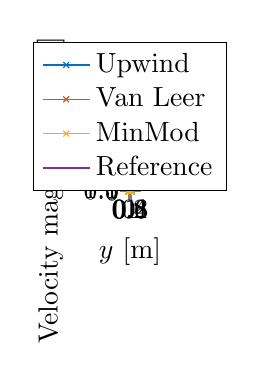
\begin{tikzpicture}

\begin{axis}[%
width=0.951\roughwidth,
height=0.75\roughheight,
at={(0\roughwidth,0\roughheight)},
scale only axis,
xmin=0,
xmax=1,
xlabel={$y$ [m]},
ymin=0,
ymax=1.5,
ylabel={Velocity magnitude [m/s]},
axis background/.style={fill=white},
legend style={at={(0.5,0.03)}, anchor=south, legend cell align=left, align=left}
]
\addplot [color=mycolor1, mark size=1.5pt, mark=x, mark options={solid, mycolor1}]
  table[row sep=crcr]{%
0	0\\
0.01	0.0254229\\
0.03	0.0771412\\
0.05	0.131431\\
0.07	0.189545\\
0.09	0.252263\\
0.11	0.319795\\
0.13	0.391594\\
0.15	0.466634\\
0.17	0.543711\\
0.19	0.621626\\
0.21	0.699267\\
0.23	0.775657\\
0.25	0.849957\\
0.27	0.921463\\
0.29	0.989594\\
0.31	1.05388\\
0.33	1.11392\\
0.35	1.16942\\
0.37	1.22012\\
0.39	1.26583\\
0.41	1.3064\\
0.43	1.34169\\
0.45	1.37161\\
0.47	1.39609\\
0.49	1.41506\\
0.51	1.42849\\
0.53	1.43632\\
0.55	1.43854\\
0.57	1.43512\\
0.59	1.42606\\
0.61	1.41134\\
0.63	1.39096\\
0.65	1.36491\\
0.67	1.3332\\
0.69	1.29582\\
0.71	1.25279\\
0.73	1.2041\\
0.75	1.14977\\
0.77	1.0898\\
0.79	1.02421\\
0.81	0.953007\\
0.83	0.876208\\
0.85	0.79383\\
0.87	0.705892\\
0.89	0.612418\\
0.91	0.513432\\
0.93	0.408963\\
0.95	0.299044\\
0.97	0.183712\\
0.99	0.063011\\
1	0\\
};
\addlegendentry{Upwind}

\addplot [color=mycolor2, mark size=1.5pt, mark=x, mark options={solid, mycolor2}]
  table[row sep=crcr]{%
0	0\\
0.01	0.0256098\\
0.03	0.0776368\\
0.05	0.132183\\
0.07	0.190504\\
0.09	0.253384\\
0.11	0.321031\\
0.13	0.392898\\
0.15	0.467961\\
0.17	0.54502\\
0.19	0.62289\\
0.21	0.700459\\
0.23	0.77675\\
0.25	0.850931\\
0.27	0.922307\\
0.29	0.990298\\
0.31	1.05443\\
0.33	1.11433\\
0.35	1.16969\\
0.37	1.22025\\
0.39	1.26584\\
0.41	1.30628\\
0.43	1.34146\\
0.45	1.37129\\
0.47	1.39566\\
0.49	1.41456\\
0.51	1.42791\\
0.53	1.43568\\
0.55	1.43786\\
0.57	1.4344\\
0.59	1.42531\\
0.61	1.41057\\
0.63	1.39018\\
0.65	1.36413\\
0.67	1.33242\\
0.69	1.29505\\
0.71	1.25203\\
0.73	1.20336\\
0.75	1.14905\\
0.77	1.08912\\
0.79	1.02356\\
0.81	0.952393\\
0.83	0.875636\\
0.85	0.793306\\
0.87	0.70542\\
0.89	0.612002\\
0.91	0.513077\\
0.93	0.408675\\
0.95	0.298828\\
0.97	0.183576\\
0.99	0.0629624\\
1	0\\
};
\addlegendentry{Van Leer}

\addplot [color=mycolor3, mark size=1.5pt, mark=x, mark options={solid, mycolor3}]
  table[row sep=crcr]{%
0	0\\
0.01	0.0255838\\
0.03	0.0775663\\
0.05	0.132074\\
0.07	0.190362\\
0.09	0.253217\\
0.11	0.320848\\
0.13	0.392711\\
0.15	0.467774\\
0.17	0.544841\\
0.19	0.622723\\
0.21	0.70031\\
0.23	0.776621\\
0.25	0.850825\\
0.27	0.92222\\
0.29	0.990231\\
0.31	1.05439\\
0.33	1.1143\\
0.35	1.16968\\
0.37	1.22026\\
0.39	1.26586\\
0.41	1.30632\\
0.43	1.34151\\
0.45	1.37134\\
0.47	1.39573\\
0.49	1.41463\\
0.51	1.42799\\
0.53	1.43577\\
0.55	1.43795\\
0.57	1.4345\\
0.59	1.42541\\
0.61	1.41067\\
0.63	1.39028\\
0.65	1.36422\\
0.67	1.33251\\
0.69	1.29514\\
0.71	1.25212\\
0.73	1.20345\\
0.75	1.14914\\
0.77	1.08919\\
0.79	1.02363\\
0.81	0.952462\\
0.83	0.8757\\
0.85	0.793364\\
0.87	0.705472\\
0.89	0.612048\\
0.91	0.513116\\
0.93	0.408706\\
0.95	0.298851\\
0.97	0.183591\\
0.99	0.0629675\\
1	0\\
};
\addlegendentry{MinMod}

\addplot [color=mycolor4]
  table[row sep=crcr]{%
0	0\\
0.00166667	0.00452198\\
0.005	0.0135298\\
0.00833333	0.0225133\\
0.0116667	0.0314839\\
0.015	0.0404525\\
0.0183333	0.0494296\\
0.0216667	0.0584251\\
0.025	0.0674484\\
0.0283333	0.0765086\\
0.0316667	0.0856141\\
0.035	0.0947727\\
0.0383333	0.103992\\
0.0416667	0.113279\\
0.045	0.122639\\
0.0483333	0.13208\\
0.0516667	0.141606\\
0.055	0.151223\\
0.0583333	0.160933\\
0.0616667	0.170742\\
0.065	0.180653\\
0.0683333	0.190669\\
0.0716667	0.200792\\
0.075	0.211024\\
0.0783333	0.221367\\
0.0816667	0.231823\\
0.085	0.242391\\
0.0883333	0.253073\\
0.0916667	0.263866\\
0.095	0.274774\\
0.0983333	0.285794\\
0.101667	0.296923\\
0.105	0.308161\\
0.108333	0.319508\\
0.111667	0.330959\\
0.115	0.342513\\
0.118333	0.354168\\
0.121667	0.365919\\
0.125	0.377765\\
0.128333	0.3897\\
0.131667	0.401723\\
0.135	0.413829\\
0.138333	0.426013\\
0.141667	0.438273\\
0.145	0.450603\\
0.148333	0.462999\\
0.151667	0.475457\\
0.155	0.487973\\
0.158333	0.50054\\
0.161667	0.513155\\
0.165	0.525812\\
0.168333	0.538508\\
0.171667	0.551237\\
0.175	0.563993\\
0.178333	0.576772\\
0.181667	0.58957\\
0.185	0.602381\\
0.188333	0.615201\\
0.191667	0.628024\\
0.195	0.640846\\
0.198333	0.653662\\
0.201667	0.666468\\
0.205	0.679258\\
0.208333	0.69203\\
0.211667	0.704776\\
0.215	0.717494\\
0.218333	0.730179\\
0.221667	0.742827\\
0.225	0.755434\\
0.228333	0.767995\\
0.231667	0.780507\\
0.235	0.792966\\
0.238333	0.805369\\
0.241667	0.81771\\
0.245	0.829988\\
0.248333	0.842198\\
0.251667	0.854338\\
0.255	0.866403\\
0.258333	0.878391\\
0.261667	0.890298\\
0.265	0.902123\\
0.268333	0.913861\\
0.271667	0.925509\\
0.275	0.937066\\
0.278333	0.948529\\
0.281667	0.959895\\
0.285	0.971162\\
0.288333	0.982327\\
0.291667	0.993388\\
0.295	1.00434\\
0.298333	1.01519\\
0.301667	1.02593\\
0.305	1.03655\\
0.308333	1.04706\\
0.311667	1.05746\\
0.315	1.06773\\
0.318333	1.07789\\
0.321667	1.08792\\
0.325	1.09784\\
0.328333	1.10763\\
0.331667	1.1173\\
0.335	1.12684\\
0.338333	1.13625\\
0.341667	1.14553\\
0.345	1.15468\\
0.348333	1.1637\\
0.351667	1.17258\\
0.355	1.18133\\
0.358333	1.18995\\
0.361667	1.19843\\
0.365	1.20677\\
0.368333	1.21498\\
0.371667	1.22305\\
0.375	1.23097\\
0.378333	1.23876\\
0.381667	1.24641\\
0.385	1.25391\\
0.388333	1.26127\\
0.391667	1.26849\\
0.395	1.27556\\
0.398333	1.28249\\
0.401667	1.28927\\
0.405	1.29591\\
0.408333	1.3024\\
0.411667	1.30875\\
0.415	1.31495\\
0.418333	1.321\\
0.421667	1.3269\\
0.425	1.33266\\
0.428333	1.33826\\
0.431667	1.34372\\
0.435	1.34902\\
0.438333	1.35417\\
0.441667	1.35918\\
0.445	1.36403\\
0.448333	1.36873\\
0.451667	1.37328\\
0.455	1.37768\\
0.458333	1.38191\\
0.461667	1.38601\\
0.465	1.38995\\
0.468333	1.39373\\
0.471667	1.39737\\
0.475	1.40085\\
0.478333	1.40417\\
0.481667	1.40735\\
0.485	1.41036\\
0.488333	1.41323\\
0.491667	1.41594\\
0.495	1.41849\\
0.498333	1.42089\\
0.501667	1.42313\\
0.505	1.42522\\
0.508333	1.42716\\
0.511667	1.42894\\
0.515	1.43056\\
0.518333	1.43202\\
0.521667	1.43334\\
0.525	1.43449\\
0.528333	1.43549\\
0.531667	1.43633\\
0.535	1.43702\\
0.538333	1.43755\\
0.541667	1.43792\\
0.545	1.43814\\
0.548333	1.4382\\
0.551667	1.4381\\
0.555	1.43785\\
0.558333	1.43744\\
0.561667	1.43687\\
0.565	1.43615\\
0.568333	1.43527\\
0.571667	1.43423\\
0.575	1.43304\\
0.578333	1.43168\\
0.581667	1.43017\\
0.585	1.4285\\
0.588333	1.42668\\
0.591667	1.4247\\
0.595	1.42256\\
0.598333	1.42026\\
0.601667	1.41781\\
0.605	1.4152\\
0.608333	1.41243\\
0.611667	1.40951\\
0.615	1.40642\\
0.618333	1.40319\\
0.621667	1.39979\\
0.625	1.39623\\
0.628333	1.39252\\
0.631667	1.38865\\
0.635	1.38462\\
0.638333	1.38044\\
0.641667	1.3761\\
0.645	1.3716\\
0.648333	1.36694\\
0.651667	1.36213\\
0.655	1.35715\\
0.658333	1.35202\\
0.661667	1.34674\\
0.665	1.34129\\
0.668333	1.33569\\
0.671667	1.32993\\
0.675	1.32402\\
0.678333	1.31794\\
0.681667	1.31171\\
0.685	1.30532\\
0.688333	1.29878\\
0.691667	1.29207\\
0.695	1.28521\\
0.698333	1.2782\\
0.701667	1.27102\\
0.705	1.26369\\
0.708333	1.2562\\
0.711667	1.24855\\
0.715	1.24075\\
0.718333	1.23279\\
0.721667	1.22467\\
0.725	1.2164\\
0.728333	1.20797\\
0.731667	1.19938\\
0.735	1.19064\\
0.738333	1.18174\\
0.741667	1.17268\\
0.745	1.16346\\
0.748333	1.15409\\
0.751667	1.14456\\
0.755	1.13488\\
0.758333	1.12504\\
0.761667	1.11504\\
0.765	1.10489\\
0.768333	1.09458\\
0.771667	1.08411\\
0.775	1.07349\\
0.778333	1.06271\\
0.781667	1.05177\\
0.785	1.04068\\
0.788333	1.02943\\
0.791667	1.01803\\
0.795	1.00647\\
0.798333	0.994758\\
0.801667	0.982888\\
0.805	0.970862\\
0.808333	0.958681\\
0.811667	0.946344\\
0.815	0.933851\\
0.818333	0.921203\\
0.821667	0.9084\\
0.825	0.895442\\
0.828333	0.882328\\
0.831667	0.86906\\
0.835	0.855636\\
0.838333	0.842058\\
0.841667	0.828325\\
0.845	0.814438\\
0.848333	0.800395\\
0.851667	0.786198\\
0.855	0.771847\\
0.858333	0.757342\\
0.861667	0.742682\\
0.865	0.727868\\
0.868333	0.712901\\
0.871667	0.697779\\
0.875	0.682504\\
0.878333	0.667075\\
0.881667	0.651492\\
0.885	0.635756\\
0.888333	0.619867\\
0.891667	0.603825\\
0.895	0.587629\\
0.898333	0.571281\\
0.901667	0.55478\\
0.905	0.538126\\
0.908333	0.521319\\
0.911667	0.504361\\
0.915	0.48725\\
0.918333	0.469987\\
0.921667	0.452572\\
0.925	0.435005\\
0.928333	0.417287\\
0.931667	0.399417\\
0.935	0.381396\\
0.938333	0.363224\\
0.941667	0.344901\\
0.945	0.326427\\
0.948333	0.307803\\
0.951667	0.289028\\
0.955	0.270103\\
0.958333	0.251028\\
0.961667	0.231803\\
0.965	0.212428\\
0.968333	0.192904\\
0.971667	0.173231\\
0.975	0.153409\\
0.978333	0.133438\\
0.981667	0.113319\\
0.985	0.0930514\\
0.988333	0.0726357\\
0.991667	0.0520722\\
0.995	0.0313611\\
0.998333	0.0105027\\
1	0\\
};
\addlegendentry{Reference}
\addplot [color=black, dashed]
  table[row sep=crcr]{%
0.1	0\\
0.1 1.5\\
};
\end{axis}
\end{tikzpicture}%
	\caption[Profile of the magnitude of the velocity in the rough channel with 
	shallow cavities at $Re=1$]{Profile of the magnitude of the velocity 
	$[\si{m/s}]$ in the rough channel with shallow cavities along the section 
	$x=\SI{8.75}{m}$, at $t=\SI{5}{s}$. $Re=1$. The region on the left of the 
	dashed line is inside the cavity.}
	\label{fig:linecompshallowlre}
\end{figure}
\begin{table}
	\centering
	\[
	\begin{array}{ccc}
	\toprule
	\text{Upwind} & \text{Van Leer} & \text{Van Alabada}\\
	\midrule
	\num{3.431e-6} & \num{2.917e-6} & \num{2.937e-6}\\
	\midrule
	\text{Min-Mod} & \text{Superbee} & \text{MC Limiter} \\ 
	\midrule
	\num{2.956e-6} & \num{2.899e-6} & \num{2.902e-6}\\
	\bottomrule
	\end{array}
	\]
	\caption[$L^2$-errors for the profile of the magnitude of the velocity in 
	the rough channel with shallow cavities at $Re=1$]{$L^2$-errors for the 
	profile of the magnitude of the velocity along a section at 
	$x=\SI{8.75}{m}$ and $t=\SI{5}{s}$ in the rough channel with shallow 
	cavities. $Re = 1$.}
	\label{tab:errshallow_lre}
\end{table}
%
\subsubsection{Deep cavities}
In the case of deep cavities we use the domain in Figure~\ref{fig:roughdomdeep} 
and we employ a uniform grid of $\num{95x70}$ cells. Again we solve until 
$T=\SI{10}{s}$, starting from an initial time-step of $\SI{e-3}{s}$. We set 
$\nu=\SI{5e-4}{m^2/s}$, so that $Re=\num{2.8e3}$. As before we compute a 
reference solution over a grid six times finer.

In Figure~\ref{fig:linecompdeep} we compare the profiles of the magnitude of 
the velocity along the section at $x=\SI{8.75}{m}$. Now the biggest differences 
are in the region inside the cavity, where the recirculation occurs. The upwind 
method, with its numerical diffusion, smooths the profile, while the TVD 
methods produce a more accurate result, even if they do not match exactly the 
reference solution. Indeed, looking at the $L^2$-errors reported in 
Table~\ref{tab:errdeep}, we see that the upwind has again the largest error, 
but the difference with the other schemes is reduced with respect to the 
previous case of shallow cavities.
\begin{figure}
	\centering
	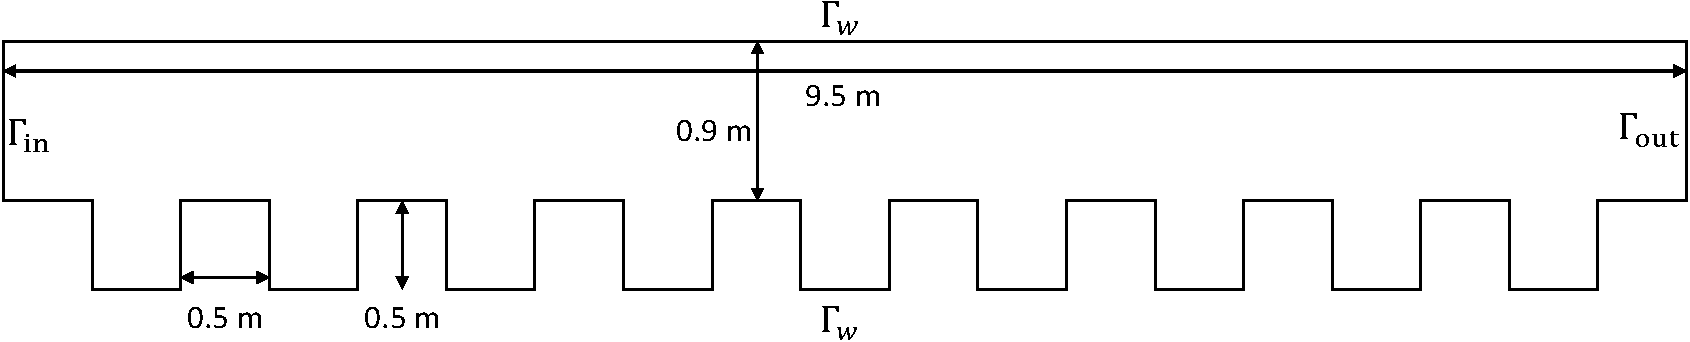
\includegraphics[width=\textwidth]{rough_domain_highstep2.pdf}
	\caption[Domain of the rough channel test with deep cavities]{Domain of the 
	rough channel test with deep cavities.}
	\label{fig:roughdomdeep}
\end{figure}
\begin{figure}
	\centering
	% This file was created by matlab2tikz.
%
\definecolor{mycolor1}{rgb}{0.00000,0.44700,0.74100}%
\definecolor{mycolor2}{rgb}{0.85000,0.32500,0.09800}%
\definecolor{mycolor3}{rgb}{0.92900,0.69400,0.12500}%
\definecolor{mycolor4}{rgb}{0.49400,0.18400,0.55600}%
%
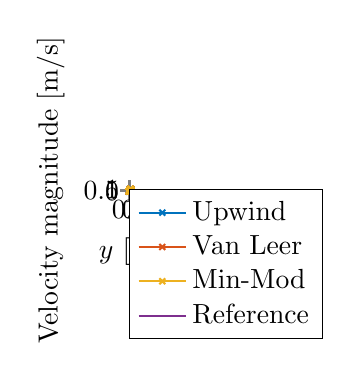
\begin{tikzpicture}

\begin{axis}[%
width=0.951\roughwidth,
height=0.75\roughheight,
at={(0\roughwidth,0\roughheight)},
scale only axis,
xmin=0,
xmax=1.4,
xlabel={$y$ [m]},
ymin=0,
ymax=1.25,
ylabel={Velocity magnitude [m/s]},
axis background/.style={fill=white},
legend style={at={(0.03,0.97)}, anchor=north west, legend cell align=left, align=left}
]

\addplot [color=mycolor1, mark size=1.5pt, mark=x, mark options={solid, mycolor1}, line width=0.75pt]
  table[row sep=crcr]{%
0	0\\
0.01	0.00885222\\
0.03	0.0227802\\
0.05	0.0327807\\
0.07	0.0393192\\
0.09	0.043122\\
0.11	0.0448784\\
0.13	0.0451341\\
0.15	0.0442874\\
0.17	0.0426208\\
0.19	0.0403378\\
0.21	0.037597\\
0.23	0.0345472\\
0.25	0.0313691\\
0.27	0.0283253\\
0.29	0.0258075\\
0.31	0.0243184\\
0.33	0.024277\\
0.35	0.0257093\\
0.37	0.0283224\\
0.39	0.0319839\\
0.41	0.0370173\\
0.43	0.044611\\
0.45	0.0576046\\
0.47	0.0818451\\
0.49	0.128213\\
0.51	0.214615\\
0.53	0.35431\\
0.55	0.509962\\
0.57	0.654372\\
0.59	0.77967\\
0.61	0.885193\\
0.63	0.971543\\
0.65	1.03985\\
0.67	1.0919\\
0.69	1.12994\\
0.71	1.15654\\
0.73	1.17426\\
0.75	1.18543\\
0.77	1.19201\\
0.79	1.19557\\
0.81	1.19723\\
0.83	1.1978\\
0.85	1.19779\\
0.87	1.19754\\
0.89	1.19723\\
0.91	1.19698\\
0.93	1.19685\\
0.95	1.19686\\
0.97	1.19703\\
0.99	1.19736\\
1.01	1.19783\\
1.03	1.19841\\
1.05	1.19906\\
1.07	1.19964\\
1.09	1.19992\\
1.11	1.19953\\
1.13	1.19783\\
1.15	1.19384\\
1.17	1.1861\\
1.19	1.17264\\
1.21	1.15086\\
1.23	1.11762\\
1.25	1.06938\\
1.27	1.00254\\
1.29	0.913831\\
1.31	0.800848\\
1.33	0.662508\\
1.35	0.499366\\
1.37	0.313659\\
1.39	0.109156\\
1.4	0\\
};
\addlegendentry{Upwind}

\addplot [color=mycolor2, mark size=1.5pt, mark=x, mark options={solid, mycolor2}, line width=0.75pt]
  table[row sep=crcr]{%
0	0\\
0.01	0.0122335\\
0.03	0.0324848\\
0.05	0.0480886\\
0.07	0.0588624\\
0.09	0.0654371\\
0.11	0.0686113\\
0.13	0.0688211\\
0.15	0.0669287\\
0.17	0.0627025\\
0.19	0.0563737\\
0.21	0.0484432\\
0.23	0.0398216\\
0.25	0.0319033\\
0.27	0.0265586\\
0.29	0.0256695\\
0.31	0.0288832\\
0.33	0.0340499\\
0.35	0.0396606\\
0.37	0.0450472\\
0.39	0.0499693\\
0.41	0.0545328\\
0.43	0.0595794\\
0.45	0.0677895\\
0.47	0.0859627\\
0.49	0.128135\\
0.51	0.214164\\
0.53	0.35562\\
0.55	0.519342\\
0.57	0.670222\\
0.59	0.798895\\
0.61	0.905422\\
0.63	0.991025\\
0.65	1.05726\\
0.67	1.10635\\
0.69	1.14101\\
0.71	1.16412\\
0.73	1.17855\\
0.75	1.18688\\
0.77	1.19113\\
0.79	1.19289\\
0.81	1.19325\\
0.83	1.1929\\
0.85	1.19227\\
0.87	1.19163\\
0.89	1.19106\\
0.91	1.19067\\
0.93	1.19044\\
0.95	1.19037\\
0.97	1.1905\\
0.99	1.19084\\
1.01	1.19135\\
1.03	1.19204\\
1.05	1.19284\\
1.07	1.19365\\
1.09	1.19427\\
1.11	1.19434\\
1.13	1.19322\\
1.15	1.1899\\
1.17	1.18285\\
1.19	1.16996\\
1.21	1.14851\\
1.23	1.11525\\
1.25	1.06662\\
1.27	0.999152\\
1.29	0.909811\\
1.31	0.796478\\
1.33	0.658286\\
1.35	0.495815\\
1.37	0.311267\\
1.39	0.108298\\
1.4	0\\
};
\addlegendentry{Van Leer}

\addplot [color=mycolor3, mark size=1.5pt, mark=x, mark options={solid, mycolor3}, line width=0.75pt]
  table[row sep=crcr]{%
0	0\\
0.01	0.0113419\\
0.03	0.0297822\\
0.05	0.0438459\\
0.07	0.0535293\\
0.09	0.0594514\\
0.11	0.0623285\\
0.13	0.0627341\\
0.15	0.0613312\\
0.17	0.0581295\\
0.19	0.0533229\\
0.21	0.0472654\\
0.23	0.040544\\
0.25	0.0340756\\
0.27	0.0291588\\
0.29	0.0272168\\
0.31	0.0284915\\
0.33	0.0317763\\
0.35	0.0359173\\
0.37	0.0402998\\
0.39	0.0446982\\
0.41	0.0493064\\
0.43	0.0551453\\
0.45	0.0648297\\
0.47	0.0848545\\
0.49	0.128268\\
0.51	0.214524\\
0.53	0.355773\\
0.55	0.518594\\
0.57	0.668691\\
0.59	0.796856\\
0.61	0.903066\\
0.63	0.988544\\
0.65	1.05485\\
0.67	1.10418\\
0.69	1.13918\\
0.71	1.16273\\
0.73	1.17764\\
0.75	1.1864\\
0.77	1.19104\\
0.79	1.19311\\
0.81	1.19369\\
0.83	1.19352\\
0.85	1.19301\\
0.87	1.19243\\
0.89	1.19193\\
0.91	1.19158\\
0.93	1.19138\\
0.95	1.19133\\
0.97	1.19148\\
0.99	1.19181\\
1.01	1.19232\\
1.03	1.19298\\
1.05	1.19375\\
1.07	1.19452\\
1.09	1.19508\\
1.11	1.19505\\
1.13	1.19379\\
1.15	1.1903\\
1.17	1.18309\\
1.19	1.17005\\
1.21	1.14852\\
1.23	1.11526\\
1.25	1.06673\\
1.27	0.999415\\
1.29	0.910241\\
1.31	0.797042\\
1.33	0.658892\\
1.35	0.496348\\
1.37	0.311635\\
1.39	0.108434\\
1.4	0\\
};
\addlegendentry{Min-Mod}

\addplot [color=mycolor4, line width=0.75pt]
  table[row sep=crcr]{%
0	0\\
0.00166667	0.00162965\\
0.005	0.00480799\\
0.00833333	0.00790634\\
0.0116667	0.0109252\\
0.015	0.013865\\
0.0183333	0.0167258\\
0.0216667	0.019508\\
0.025	0.022212\\
0.0283333	0.0248383\\
0.0316667	0.0273878\\
0.035	0.0298613\\
0.0383333	0.03226\\
0.0416667	0.0345853\\
0.045	0.0368385\\
0.0483333	0.0390211\\
0.0516667	0.0411348\\
0.055	0.0431809\\
0.0583333	0.045161\\
0.0616667	0.0470764\\
0.065	0.0489283\\
0.0683333	0.0507176\\
0.0716667	0.0524452\\
0.075	0.0541115\\
0.0783333	0.055717\\
0.0816667	0.0572619\\
0.085	0.0587457\\
0.0883333	0.0601683\\
0.0916667	0.0615291\\
0.095	0.0628271\\
0.0983333	0.0640617\\
0.101667	0.0652316\\
0.105	0.0663357\\
0.108333	0.0673728\\
0.111667	0.0683414\\
0.115	0.0692403\\
0.118333	0.070068\\
0.121667	0.0708231\\
0.125	0.0715044\\
0.128333	0.0721104\\
0.131667	0.0726401\\
0.135	0.0730923\\
0.138333	0.0734658\\
0.141667	0.0737601\\
0.145	0.0739741\\
0.148333	0.0741073\\
0.151667	0.0741594\\
0.155	0.0741298\\
0.158333	0.0740188\\
0.161667	0.0738262\\
0.165	0.0735523\\
0.168333	0.0731975\\
0.171667	0.0727624\\
0.175	0.0722478\\
0.178333	0.0716544\\
0.181667	0.0709837\\
0.185	0.0702367\\
0.188333	0.0694149\\
0.191667	0.0685199\\
0.195	0.0675533\\
0.198333	0.0665172\\
0.201667	0.0654135\\
0.205	0.0642444\\
0.208333	0.0630124\\
0.211667	0.0617197\\
0.215	0.0603692\\
0.218333	0.0589636\\
0.221667	0.0575058\\
0.225	0.055999\\
0.228333	0.0544466\\
0.231667	0.0528522\\
0.235	0.0512197\\
0.238333	0.0495534\\
0.241667	0.0478579\\
0.245	0.0461384\\
0.248333	0.0444006\\
0.251667	0.042651\\
0.255	0.0408971\\
0.258333	0.0391474\\
0.261667	0.0374118\\
0.265	0.0357016\\
0.268333	0.0340304\\
0.271667	0.032414\\
0.275	0.0308707\\
0.278333	0.0294217\\
0.281667	0.0280915\\
0.285	0.026907\\
0.288333	0.025897\\
0.291667	0.0250911\\
0.295	0.0245166\\
0.298333	0.0241958\\
0.301667	0.0241434\\
0.305	0.024363\\
0.308333	0.0248475\\
0.311667	0.0255795\\
0.315	0.0265348\\
0.318333	0.0276856\\
0.321667	0.0290029\\
0.325	0.0304586\\
0.328333	0.0320267\\
0.331667	0.0336841\\
0.335	0.0354105\\
0.338333	0.0371883\\
0.341667	0.0390024\\
0.345	0.0408399\\
0.348333	0.0426898\\
0.351667	0.0445425\\
0.355	0.04639\\
0.358333	0.048225\\
0.361667	0.0500416\\
0.365	0.0518343\\
0.368333	0.0535986\\
0.371667	0.0553303\\
0.375	0.0570259\\
0.378333	0.0586824\\
0.381667	0.060297\\
0.385	0.0618676\\
0.388333	0.0633923\\
0.391667	0.0648697\\
0.395	0.0662986\\
0.398333	0.0676785\\
0.401667	0.0690093\\
0.405	0.0702916\\
0.408333	0.0715265\\
0.411667	0.072716\\
0.415	0.0738628\\
0.418333	0.0749713\\
0.421667	0.076047\\
0.425	0.0770969\\
0.428333	0.0781306\\
0.431667	0.0791597\\
0.435	0.0801992\\
0.438333	0.0812674\\
0.441667	0.0823869\\
0.445	0.0835853\\
0.448333	0.084896\\
0.451667	0.0863585\\
0.455	0.08802\\
0.458333	0.0899355\\
0.461667	0.0921692\\
0.465	0.0947941\\
0.468333	0.0978929\\
0.471667	0.101558\\
0.475	0.105891\\
0.478333	0.111\\
0.481667	0.117001\\
0.485	0.124015\\
0.488333	0.13216\\
0.491667	0.141554\\
0.495	0.152307\\
0.498333	0.164518\\
0.501667	0.178267\\
0.505	0.193612\\
0.508333	0.210581\\
0.511667	0.229172\\
0.515	0.249346\\
0.518333	0.271026\\
0.521667	0.294097\\
0.525	0.318416\\
0.528333	0.3438\\
0.531667	0.370031\\
0.535	0.396864\\
0.538333	0.42408\\
0.541667	0.451482\\
0.545	0.478885\\
0.548333	0.506133\\
0.551667	0.533085\\
0.555	0.559629\\
0.558333	0.585678\\
0.561667	0.611162\\
0.565	0.636036\\
0.568333	0.660269\\
0.571667	0.683845\\
0.575	0.706758\\
0.578333	0.729008\\
0.581667	0.750601\\
0.585	0.771545\\
0.588333	0.79185\\
0.591667	0.811525\\
0.595	0.83058\\
0.598333	0.849024\\
0.601667	0.866863\\
0.605	0.884107\\
0.608333	0.900759\\
0.611667	0.916826\\
0.615	0.932313\\
0.618333	0.947225\\
0.621667	0.961569\\
0.625	0.975348\\
0.628333	0.988573\\
0.631667	1.00125\\
0.635	1.01338\\
0.638333	1.02498\\
0.641667	1.03605\\
0.645	1.04661\\
0.648333	1.05667\\
0.651667	1.06623\\
0.655	1.07531\\
0.658333	1.08392\\
0.661667	1.09207\\
0.665	1.09978\\
0.668333	1.10705\\
0.671667	1.11391\\
0.675	1.12035\\
0.678333	1.12641\\
0.681667	1.13209\\
0.685	1.1374\\
0.688333	1.14237\\
0.691667	1.147\\
0.695	1.15131\\
0.698333	1.15531\\
0.701667	1.15901\\
0.705	1.16244\\
0.708333	1.1656\\
0.711667	1.16851\\
0.715	1.17118\\
0.718333	1.17363\\
0.721667	1.17586\\
0.725	1.17789\\
0.728333	1.17974\\
0.731667	1.18141\\
0.735	1.18291\\
0.738333	1.18425\\
0.741667	1.18546\\
0.745	1.18653\\
0.748333	1.18747\\
0.751667	1.18831\\
0.755	1.18903\\
0.758333	1.18966\\
0.761667	1.1902\\
0.765	1.19066\\
0.768333	1.19104\\
0.771667	1.19135\\
0.775	1.19161\\
0.778333	1.19181\\
0.781667	1.19195\\
0.785	1.19206\\
0.788333	1.19212\\
0.791667	1.19214\\
0.795	1.19214\\
0.798333	1.19211\\
0.801667	1.19205\\
0.805	1.19197\\
0.808333	1.19188\\
0.811667	1.19177\\
0.815	1.19164\\
0.818333	1.19151\\
0.821667	1.19136\\
0.825	1.19121\\
0.828333	1.19106\\
0.831667	1.1909\\
0.835	1.19073\\
0.838333	1.19057\\
0.841667	1.19041\\
0.845	1.19025\\
0.848333	1.19009\\
0.851667	1.18993\\
0.855	1.18977\\
0.858333	1.18962\\
0.861667	1.18947\\
0.865	1.18933\\
0.868333	1.18919\\
0.871667	1.18906\\
0.875	1.18893\\
0.878333	1.18881\\
0.881667	1.18869\\
0.885	1.18858\\
0.888333	1.18847\\
0.891667	1.18838\\
0.895	1.18828\\
0.898333	1.1882\\
0.901667	1.18812\\
0.905	1.18804\\
0.908333	1.18797\\
0.911667	1.18791\\
0.915	1.18786\\
0.918333	1.18781\\
0.921667	1.18776\\
0.925	1.18773\\
0.928333	1.1877\\
0.931667	1.18767\\
0.935	1.18765\\
0.938333	1.18764\\
0.941667	1.18763\\
0.945	1.18763\\
0.948333	1.18764\\
0.951667	1.18765\\
0.955	1.18767\\
0.958333	1.18769\\
0.961667	1.18772\\
0.965	1.18776\\
0.968333	1.1878\\
0.971667	1.18785\\
0.975	1.1879\\
0.978333	1.18797\\
0.981667	1.18803\\
0.985	1.18811\\
0.988333	1.18818\\
0.991667	1.18827\\
0.995	1.18836\\
0.998333	1.18846\\
1.00167	1.18856\\
1.005	1.18867\\
1.00833	1.18879\\
1.01167	1.18891\\
1.015	1.18904\\
1.01833	1.18917\\
1.02167	1.18931\\
1.025	1.18946\\
1.02833	1.18961\\
1.03167	1.18977\\
1.035	1.18993\\
1.03833	1.1901\\
1.04167	1.19027\\
1.045	1.19045\\
1.04833	1.19063\\
1.05167	1.19081\\
1.055	1.191\\
1.05833	1.19119\\
1.06167	1.19139\\
1.065	1.19158\\
1.06833	1.19177\\
1.07167	1.19197\\
1.075	1.19216\\
1.07833	1.19235\\
1.08167	1.19253\\
1.085	1.19271\\
1.08833	1.19288\\
1.09167	1.19305\\
1.095	1.1932\\
1.09833	1.19333\\
1.10167	1.19345\\
1.105	1.19355\\
1.10833	1.19362\\
1.11167	1.19367\\
1.115	1.19369\\
1.11833	1.19368\\
1.12167	1.19363\\
1.125	1.19353\\
1.12833	1.19338\\
1.13167	1.19319\\
1.135	1.19293\\
1.13833	1.1926\\
1.14167	1.1922\\
1.145	1.19172\\
1.14833	1.19115\\
1.15167	1.19049\\
1.155	1.18971\\
1.15833	1.18883\\
1.16167	1.18782\\
1.165	1.18667\\
1.16833	1.18538\\
1.17167	1.18393\\
1.175	1.18231\\
1.17833	1.18051\\
1.18167	1.17852\\
1.185	1.17632\\
1.18833	1.17389\\
1.19167	1.17123\\
1.195	1.16832\\
1.19833	1.16515\\
1.20167	1.1617\\
1.205	1.15794\\
1.20833	1.15388\\
1.21167	1.14949\\
1.215	1.14475\\
1.21833	1.13965\\
1.22167	1.13417\\
1.225	1.12829\\
1.22833	1.12201\\
1.23167	1.11529\\
1.235	1.10812\\
1.23833	1.1005\\
1.24167	1.09239\\
1.245	1.08378\\
1.24833	1.07466\\
1.25167	1.06502\\
1.255	1.05483\\
1.25833	1.04408\\
1.26167	1.03276\\
1.265	1.02085\\
1.26833	1.00835\\
1.27167	0.995228\\
1.275	0.981485\\
1.27833	0.967108\\
1.28167	0.952085\\
1.285	0.936409\\
1.28833	0.92007\\
1.29167	0.903062\\
1.295	0.885377\\
1.29833	0.867011\\
1.30167	0.847959\\
1.305	0.828218\\
1.30833	0.807786\\
1.31167	0.786662\\
1.315	0.764846\\
1.31833	0.742339\\
1.32167	0.719144\\
1.325	0.695264\\
1.32833	0.670704\\
1.33167	0.645471\\
1.335	0.619571\\
1.33833	0.593012\\
1.34167	0.565805\\
1.345	0.537959\\
1.34833	0.509487\\
1.35167	0.480401\\
1.355	0.450714\\
1.35833	0.420443\\
1.36167	0.389601\\
1.365	0.358207\\
1.36833	0.326277\\
1.37167	0.29383\\
1.375	0.260885\\
1.37833	0.227463\\
1.38167	0.193583\\
1.385	0.159268\\
1.38833	0.124538\\
1.39167	0.0894149\\
1.395	0.0539223\\
1.39833	0.0180823\\
1.4	0\\
};
\addlegendentry{Reference}
\addplot [color=black, dashed, line width=0.75pt]
  table[row sep=crcr]{%
0.5	0\\
0.5 1.25\\
};
\end{axis}
\end{tikzpicture}%
	\caption[Profile of the magnitude of the velocity in the rough channel with 
	deep cavities at $Re=\num{2.8e3}$]{Profile of the magnitude of the velocity 
		$[\si{m/s}]$ in the rough channel with deep cavities along the section 
		$x=\SI{8.75}{m}$, at $t=\SI{10}{s}$. $Re=\num{2.8e3}$. The region on 
		the 
		left of the dashed line is inside the cavity.}
	\label{fig:linecompdeep}
\end{figure}
\begin{table}
	\centering
	\[
	\begin{array}{ccc}
	\toprule
	\text{Upwind} & \text{Van Leer} & \text{Van Alabada}\\
	\midrule
	\num{3.180e-4} & \num{5.862e-5} & \num{6.900e-5}\\
	\midrule
	\text{Min-Mod} & \text{Superbee} & \text{MC Limiter} \\
	\midrule
	\num{8.579e-5} & \num{7.883e-5} & \num{5.584e-5}\\
	\bottomrule
	\end{array}
	\]
	\caption[$L^2$-errors for the profile of the magnitude of the velocity in 
	the rough channel with deep cavities]{$L^2$-errors for the profile of the 
	magnitude of the velocity along a section at $x=\SI{8.75}{m}$ and 
	$t=\SI{10}{s}$ in the rough channel with deep cavities. $Re = \num{2.8e3}$.}
	\label{tab:errdeep}
\end{table}
%
\section{RANS tests}
\subsection{Backward facing step}
%The NASA LaRC CFD code CFL3D uses:
%\begin{itemize}
%	\item free-stream turbulence intensity = 0.061\%
%	\item free-stream turbulent viscosity (relative to laminar) = 0.009
%	\item in this case the simulations were \emph{quasi-steady}, i.e. the 
%	solution does not converge readily to a steady state result when a refined 
%	grid is used. However, when run-time accurately, the solution settles down 
%	and becomes reasonably steady (quasi-steady).
%	\item The code is for compressible flows at ``essentially incompressible" 
%	conditions of M=0.128. There may be a very small influence of 
%	compressibility.
%	\item non-dimensional CFD code
%	\item first order turbulence advection in the turbulence transport equations
%	\item Neglects two terms that are zero for incompressible flows
%	\item implicit time advancement (also second order)
%	\item Central differencing in Space? Non lo dice cosa usa, inoltre secondo 
%	me non usa una staggered grid.
%\end{itemize}
\subsection{Cavities mutual influence}
%An easy result.
\section{Coupled test}
\subsection{Cavities coupled with the porous-medium}
%A more complex result.